\documentclass[tikz]{standalone}

\usetikzlibrary{arrows.meta,fit,positioning}

\begin{document}
	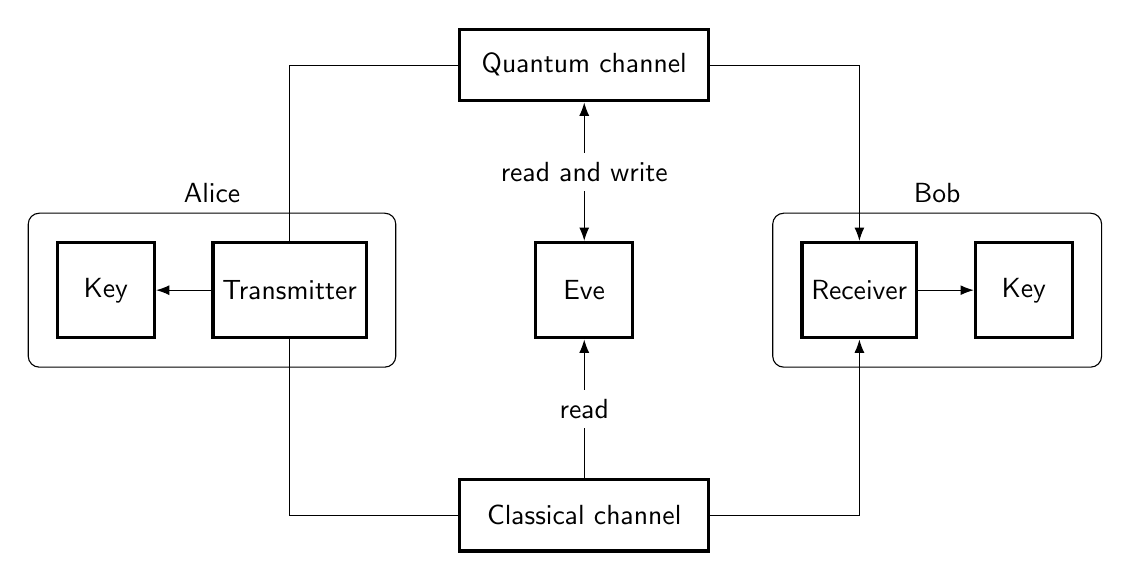
\begin{tikzpicture}[
		block/.style={draw, very thick, fill=white, minimum height=8ex, minimum width=3.5em},
		party/.style={draw, rounded corners, inner xsep=1em, inner ysep=1em},
		channel/.style={block, minimum height=6ex, minimum width=9em},
	]
		\node (ka) [block] {\textsf{Key}};
		\node (tx) [block, right=2em of ka] {\textsf{Transmitter}};
		\node [party, fit=(ka) (tx), label=\textsf{Alice}] (alice) {};
		\node [block, right=6em of tx] (eve) {\textsf{Eve}};
		\node (rx) [block, right=6em of eve] {\textsf{Receiver}};
		\node (kb) [block, right=2em of rx] {\textsf{Key}};
		\node (bob) [party, fit=(rx) (kb), label={\textsf{Bob}}] {};
		
		\node (qch) [channel, above=5em of eve] {\textsf{Quantum channel}};
		\node (cch) [channel, below=5em of eve, minimum height=6ex, minimum width=9em] {\textsf{Classical channel}};
		
		\draw[-Latex] (tx.north) -- (tx.north|-qch) -- (qch) -- (qch-|rx.north) -- (rx.north);
		\draw[-Latex] (tx.south) -- (tx.south|-cch) -- (cch) -- (cch-|rx.south) -- (rx.south);
		
		\draw[Latex-Latex] (eve) -- (qch) node[midway, fill=white]{\textsf{read and write}};
		\draw[Latex-] (eve) -- (cch) node[midway, fill=white]{\textsf{read}};
		
		\draw[-Latex] (tx) -- (ka);
		\draw[-Latex] (rx) -- (kb);
	\end{tikzpicture}
\end{document}
